
\section{Architektur}
\label{sec:Architektur}
% Vorgehen nach C4 Modell
In diesem Kapitel wird die Architektur unserer Applikation und die Schnittstellen zu den Umsystemen besprochen. Als Anhaltspunkt wird das C4 Modell \cite{c4model} von Simon Brown verwendet. In einem ersten Schritt wird unsere Applikation in den Kontext des grösseren Systems gesetzt. Anschliessend teilen wir das System \emph{PlazaRoute} in einzelne Container und den zentralen Container \emph{Plaza Routing} in einzelne Komponenten auf.

\subsection{Systemkontext}
\label{architektur:Systemkontext}

\begin{figure}[ht]
\centering
% TODO: Grafik zuschneiden
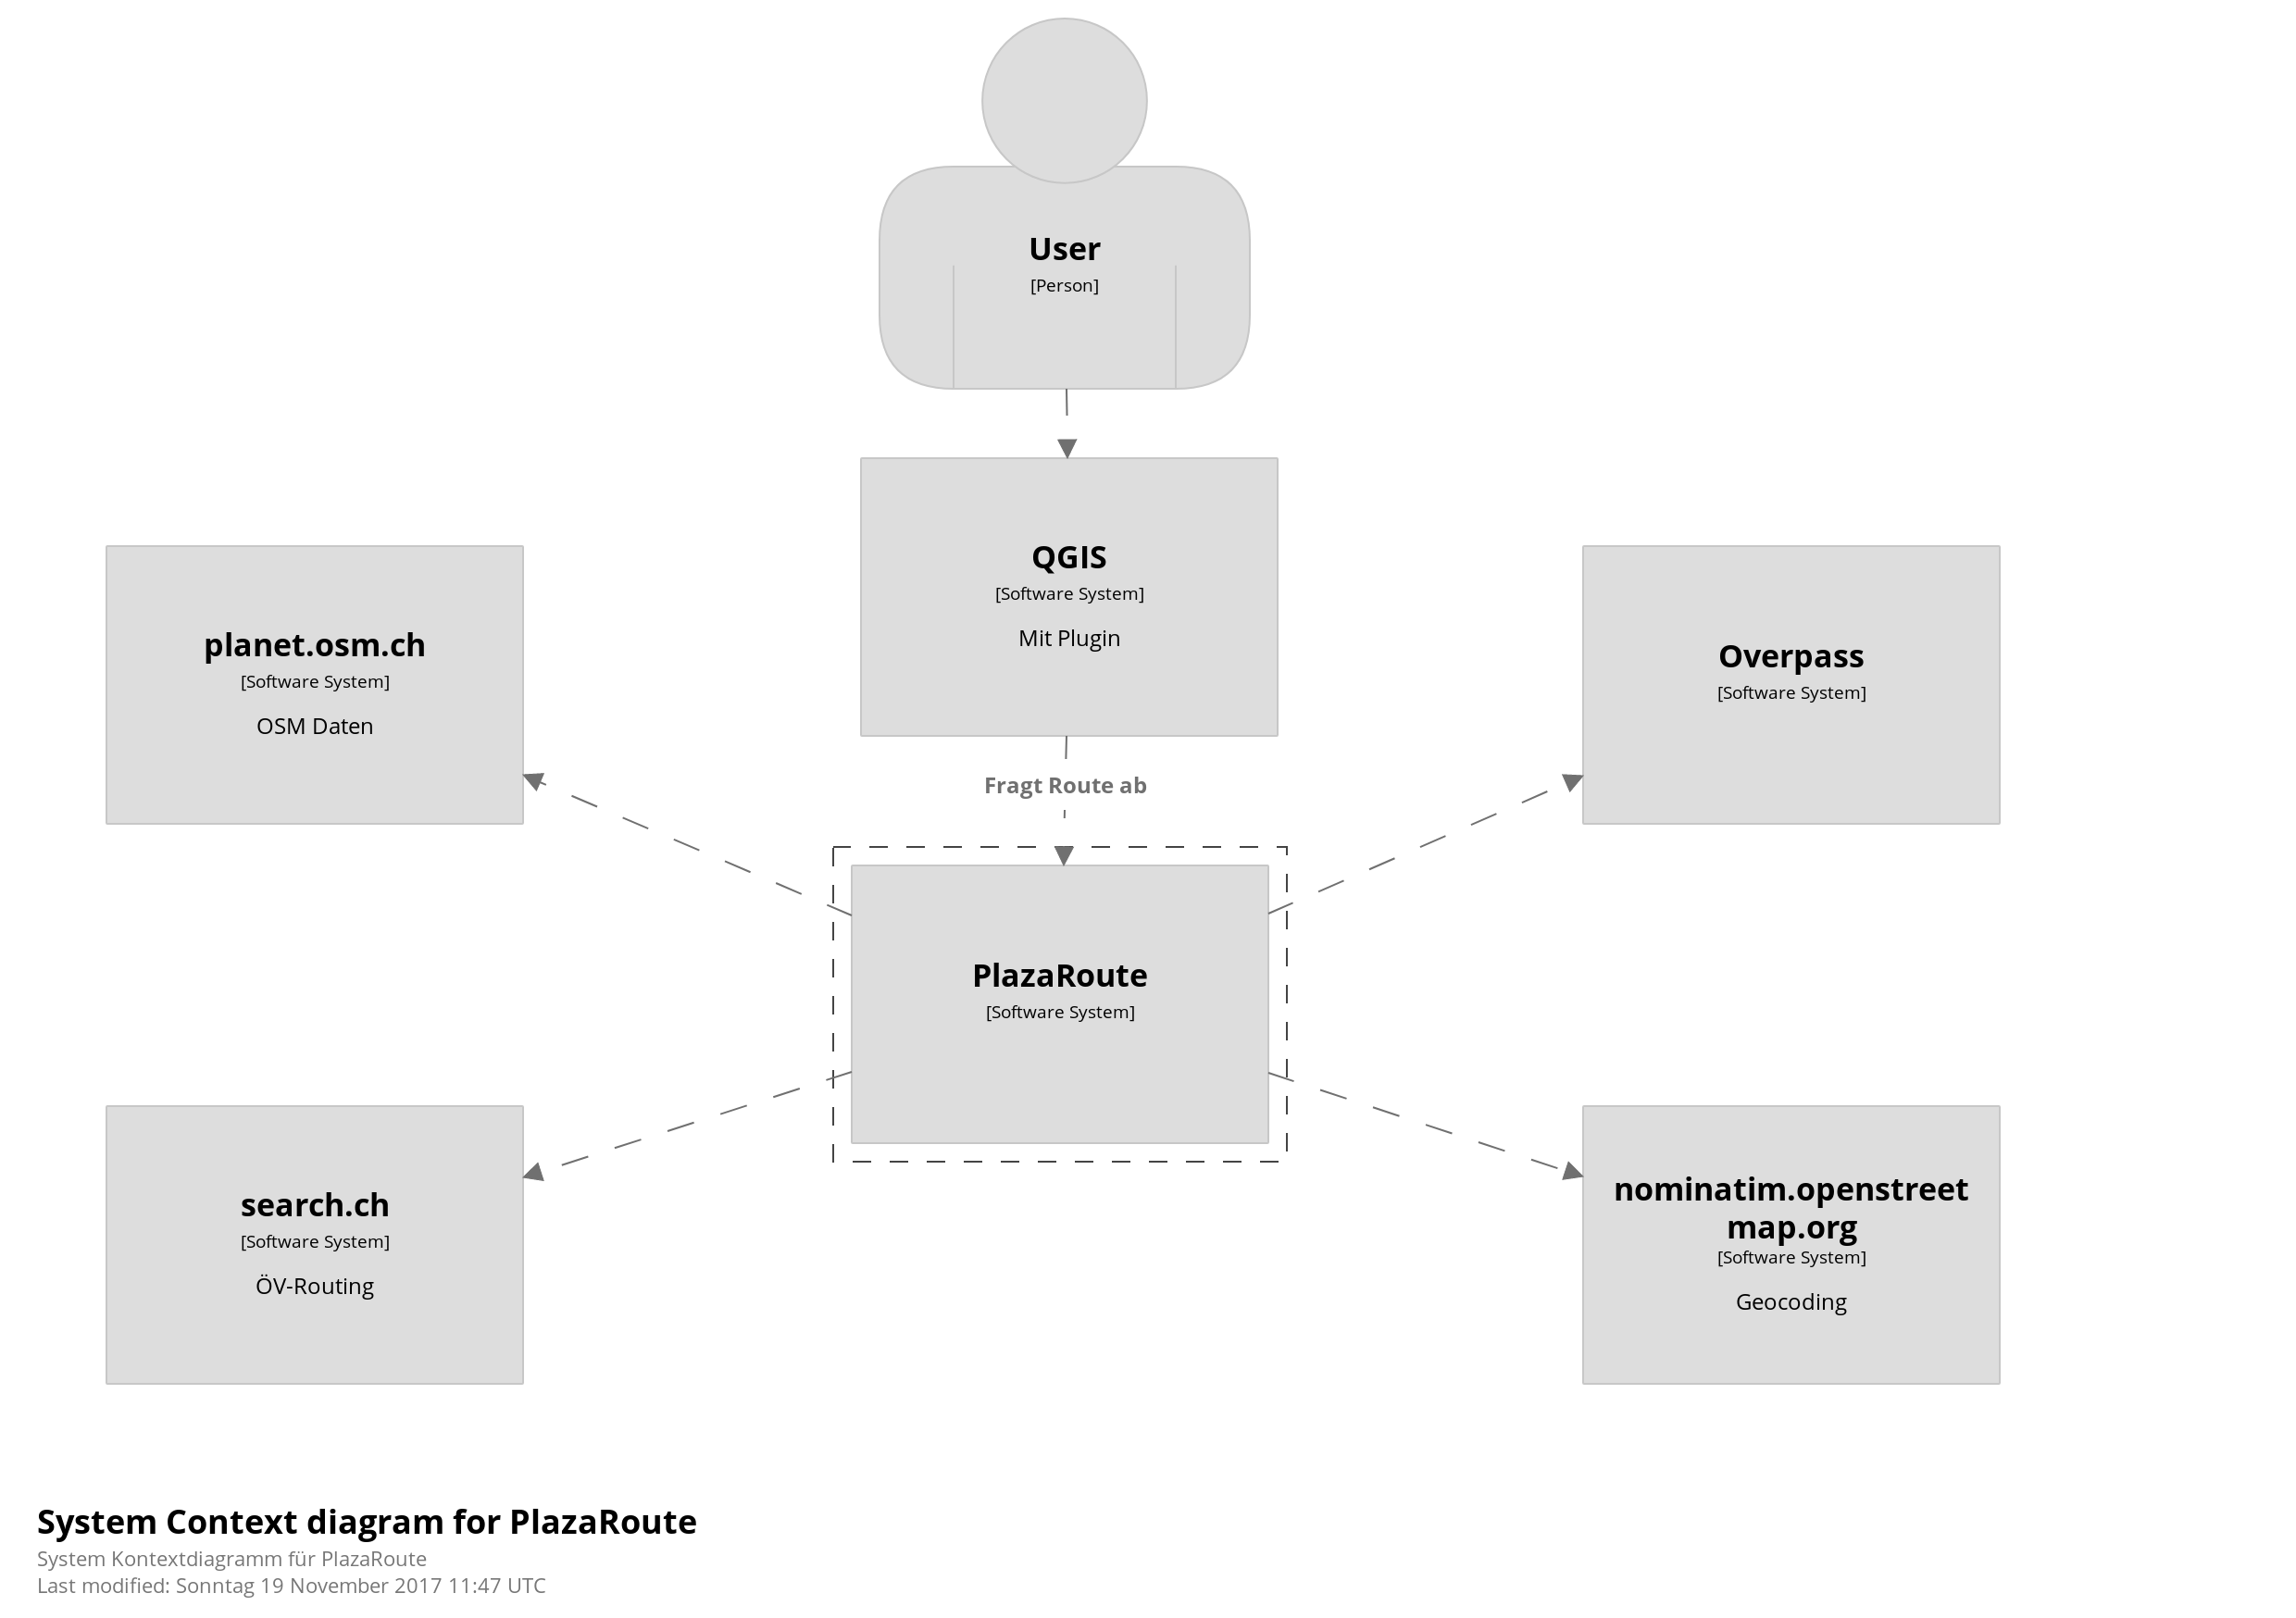
\includegraphics[width=1\linewidth]{projectdoc/img/system-context_diagram.png}
\caption[System Kontext Diagramm]{System PlazaRoute im Kontext mit Umsystemen; Grafik erstellt mit \emph{Structurizr Express}\cite{structurizr}}
\label{fig:system_context_diagram}
\end{figure}

Abbildung \ref{fig:system_context_diagram} zeigt das System PlazaRoute mit den Umsystemen auf.

Der User bedient die QGIS Desktop Applikation mit dem von uns entwickelten Plugin. Dieses leitet die die Eingabe der Start- und Zielkoordinaten an das System PlazaRoute weiter. Als Antwort sendet PlazaRoute eine Routenbeschreibung an das QGIS-Plugin zurück, das es im QGIS darstellt.

\subsection{QGIS Plugin}
\label{architektur:QGIS Plugin}
Das QGIS-Plugin ist unabhängig vom System PlazaRoute und läuft auf dem Client des Benutzers. Die Kommunikation mit dem Container Plaza Routing erfolgt mit HTTPS.
% TODO: Mehr Detail, sobald wir mehr wissen

\subsection{PlazaRoute Container}
\label{architektur:PlazaRoute Container}

\begin{figure}[ht]
    \centering
    % TODO: Grafik zuschneiden
    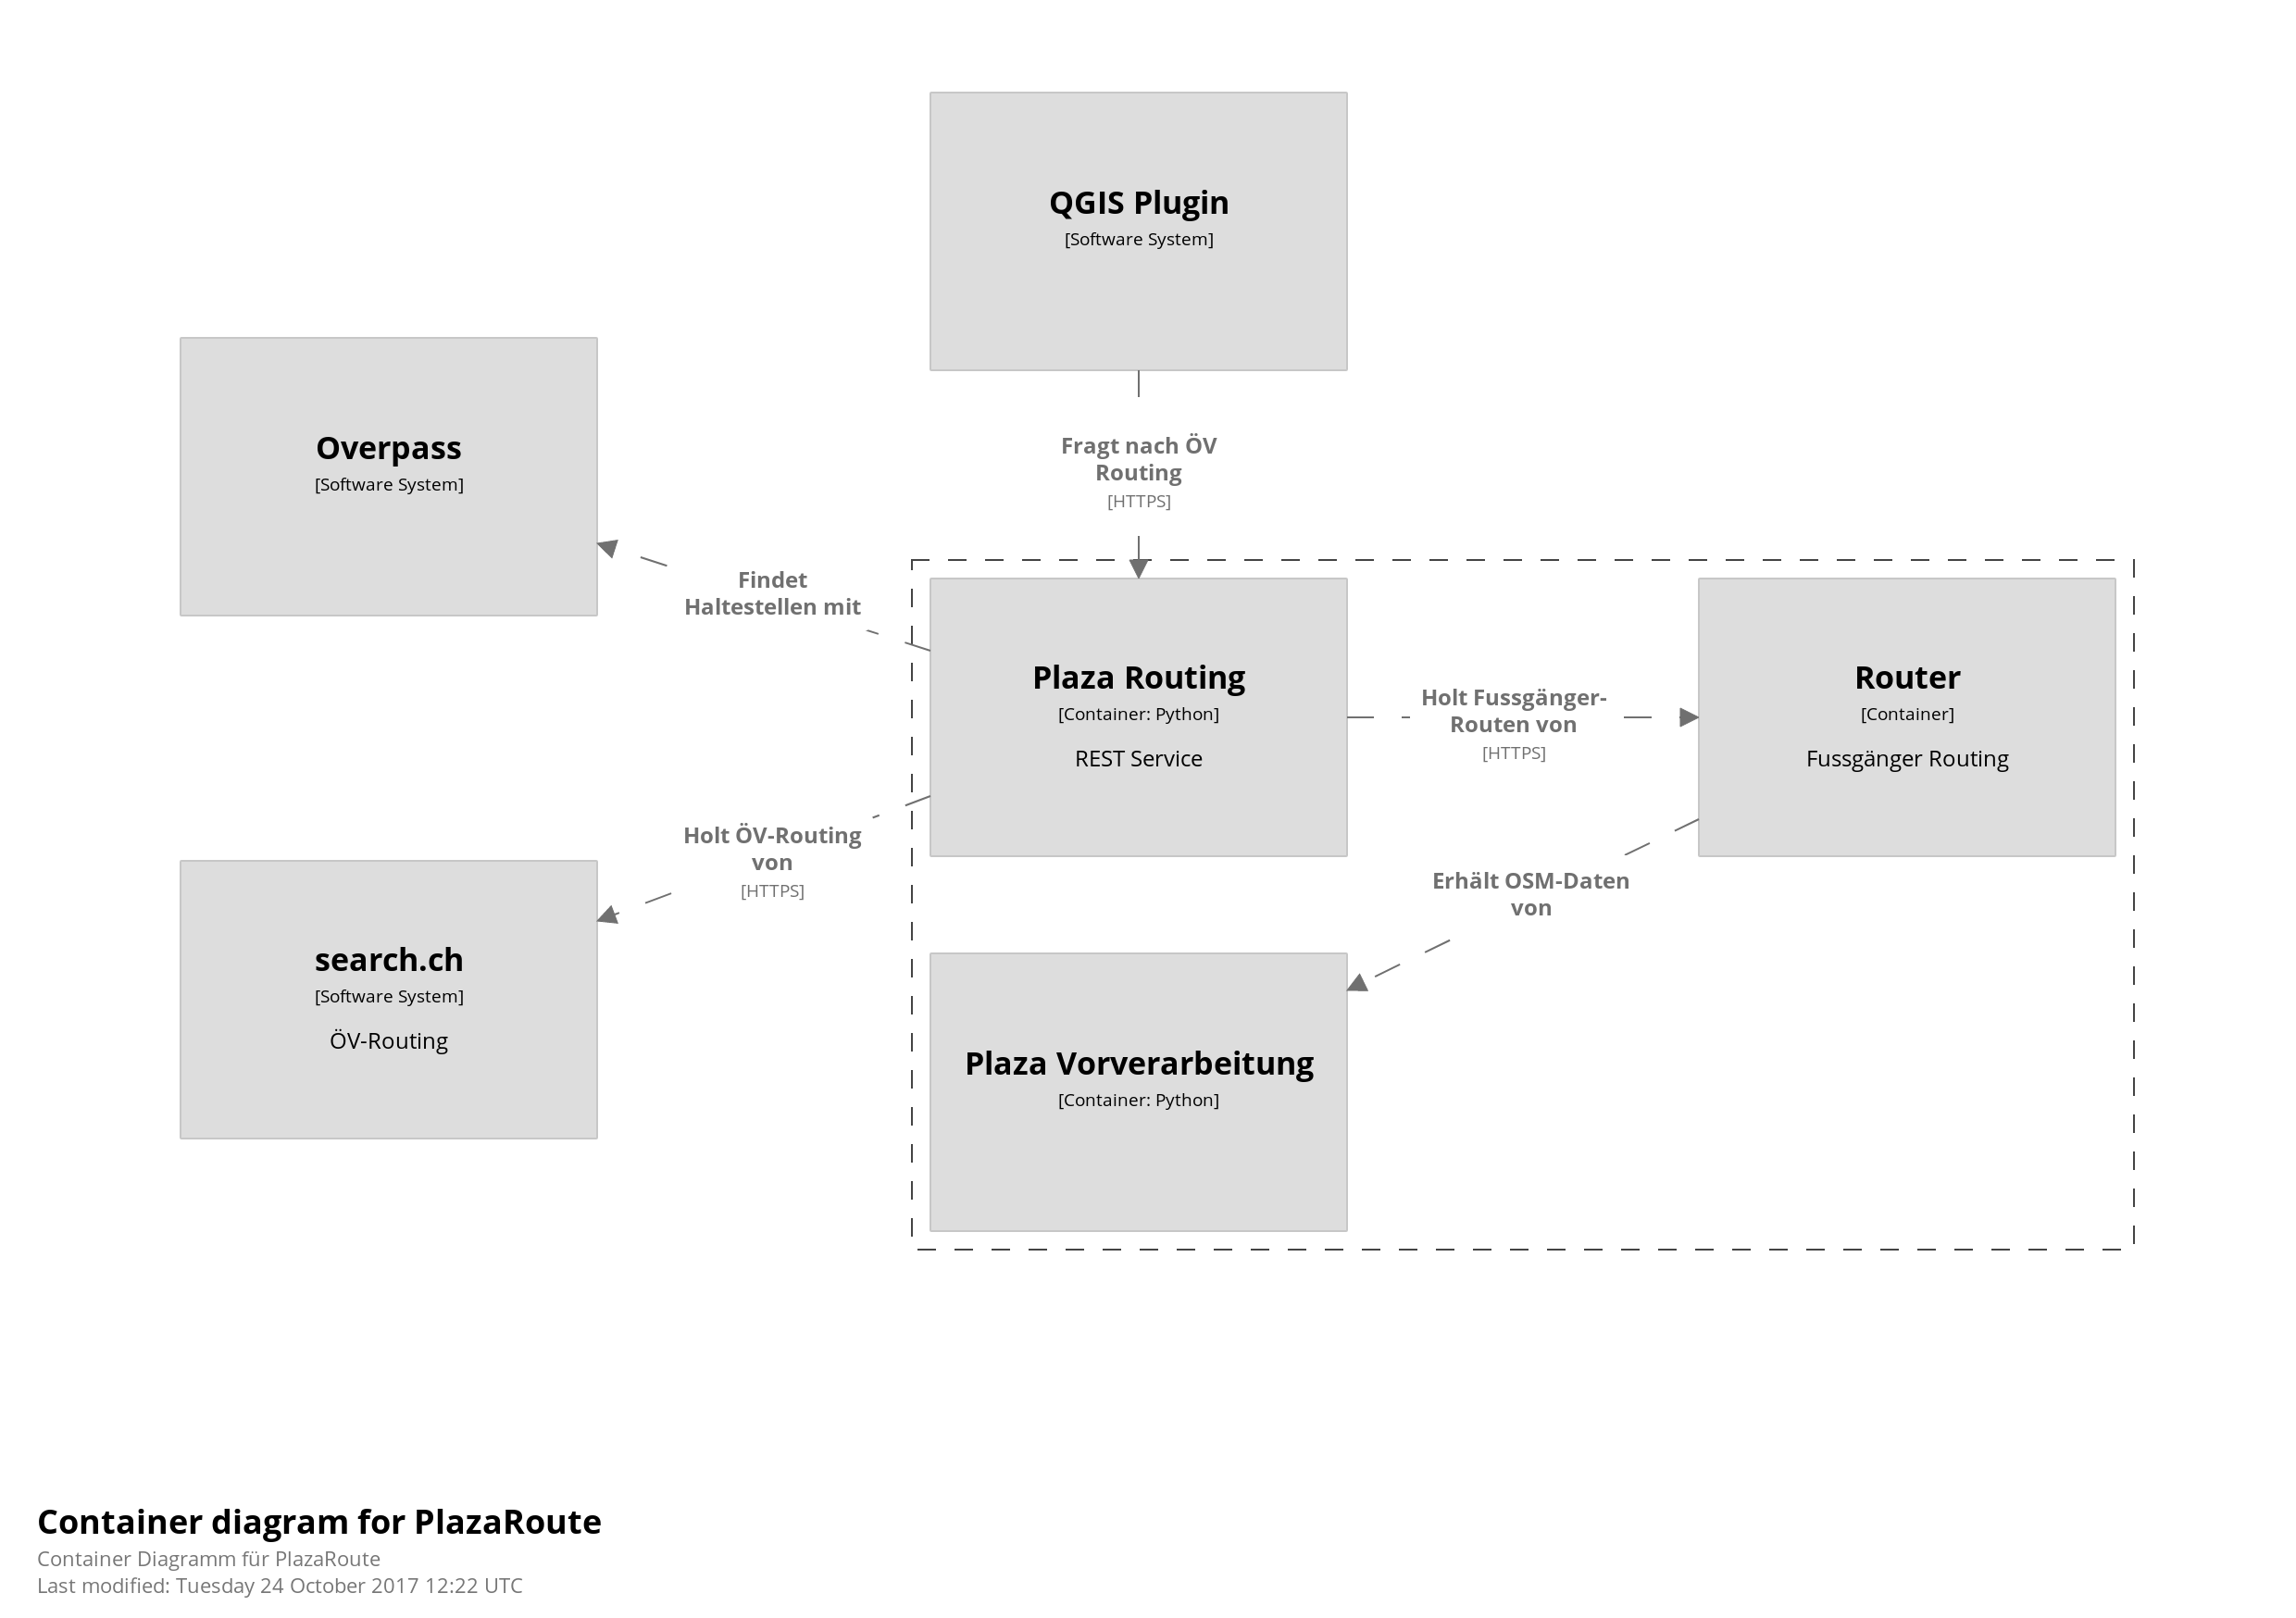
\includegraphics[width=1\linewidth]{projectdoc/img/container_diagram.png}
    \caption[Container Diagramm]{Container Diagramm von PlazaRoute; Grafik erstellt mit \emph{Structurizr Express}\cite{structurizr}}
    \label{fig:container_diagram}
    \end{figure}    

In Abbildung \ref{fig:container_diagram} zoomen wir in das System PlazaRoute hinein und teilen es in drei Container auf, die logisch voneinander getrennt sind. So könnten die Container auch verteilt deployed werden.

In den nachfolgenden Abschnitten werden die drei Container näher beleuchtet.


\subsubsection{Plaza Vorverarbeitung}
\label{architektur:Plaza Vorverarbeitung}

Bevor die \nameref{architektur:Routing-Engine} ihre Routing-Funktion ausführen kann, muss diese zuerst aus dem \ac{OSM}-Datensatz einen Routing-Graph generieren. Unsere Hauptaufgabe besteht darin, diesen Routing-Graphen für Fussgänger-Routing über Flächen zu optimieren. Ein Ansatz wäre, den Graphen nach dem Generieren zu verändern. Dies ist aber schwer realisierbar, da die meisten Routing-Engines die Graphen in eigenen (binären) Datenstrukturen ablegen. So wär unsere Implementation auch stark an eine einzelne Routing-Engine gekoppelt.

Ein zweiter Ansatz die Integration unserer Optimierung in die Verarbeitung der Routing-Engines selbst. Auch da wären wir wieder stark an eine spezifische Routing-Engine gekoppelt.
Wir haben uns stattdessen entschieden, beim Input der \ac{OSM}-Daten anzusetzen. Dazu werden die Rohdaten zuerst eingelesen und nach Fussgänger-Flächen abgesucht (\nameref{par:OSM Importer}). Mit unserem Algorithmus werden neue Fusswege eingetragen (\nameref{par:Plaza Optimizer}). Diese neu erzeugten Kartendaten werden dann wieder mit den ursprünglichen Rohdaten verschmelzt (\nameref{par:OSM Merger}). Erst dann generiert die Routing-Engine daraus den Routing-Graphen. Das Vorgehen ist in Abbildung \ref{fig:workflow_vorverarbeitung} schematisch aufgezeigt.

Abbildung \ref{fig:component_diagram_vorverarbeitung} zeigt die einzelnen Komponenten für die Vorverarbeitung der \ac{OSM}-Daten auf.


\begin{figure}[ht]
    \centering
    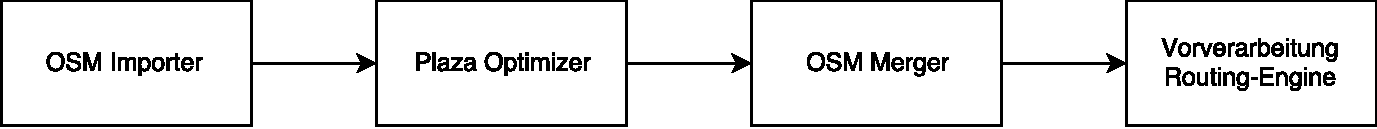
\includegraphics[width=1\linewidth]{projectdoc/img/workflow_vorverarbeitung.pdf}
    \caption[Ablauf Vorverarbeitung]{Ablauf der Vorverarbeitung der \ac{OSM}-Daten bis zur Übergabe an die Routing-Engine; Grafik erstellt mit \emph{draw.io}}
    \label{fig:workflow_vorverarbeitung}
\end{figure}
    

\begin{figure}[ht]
\centering
% TODO: Grafik zuschneiden
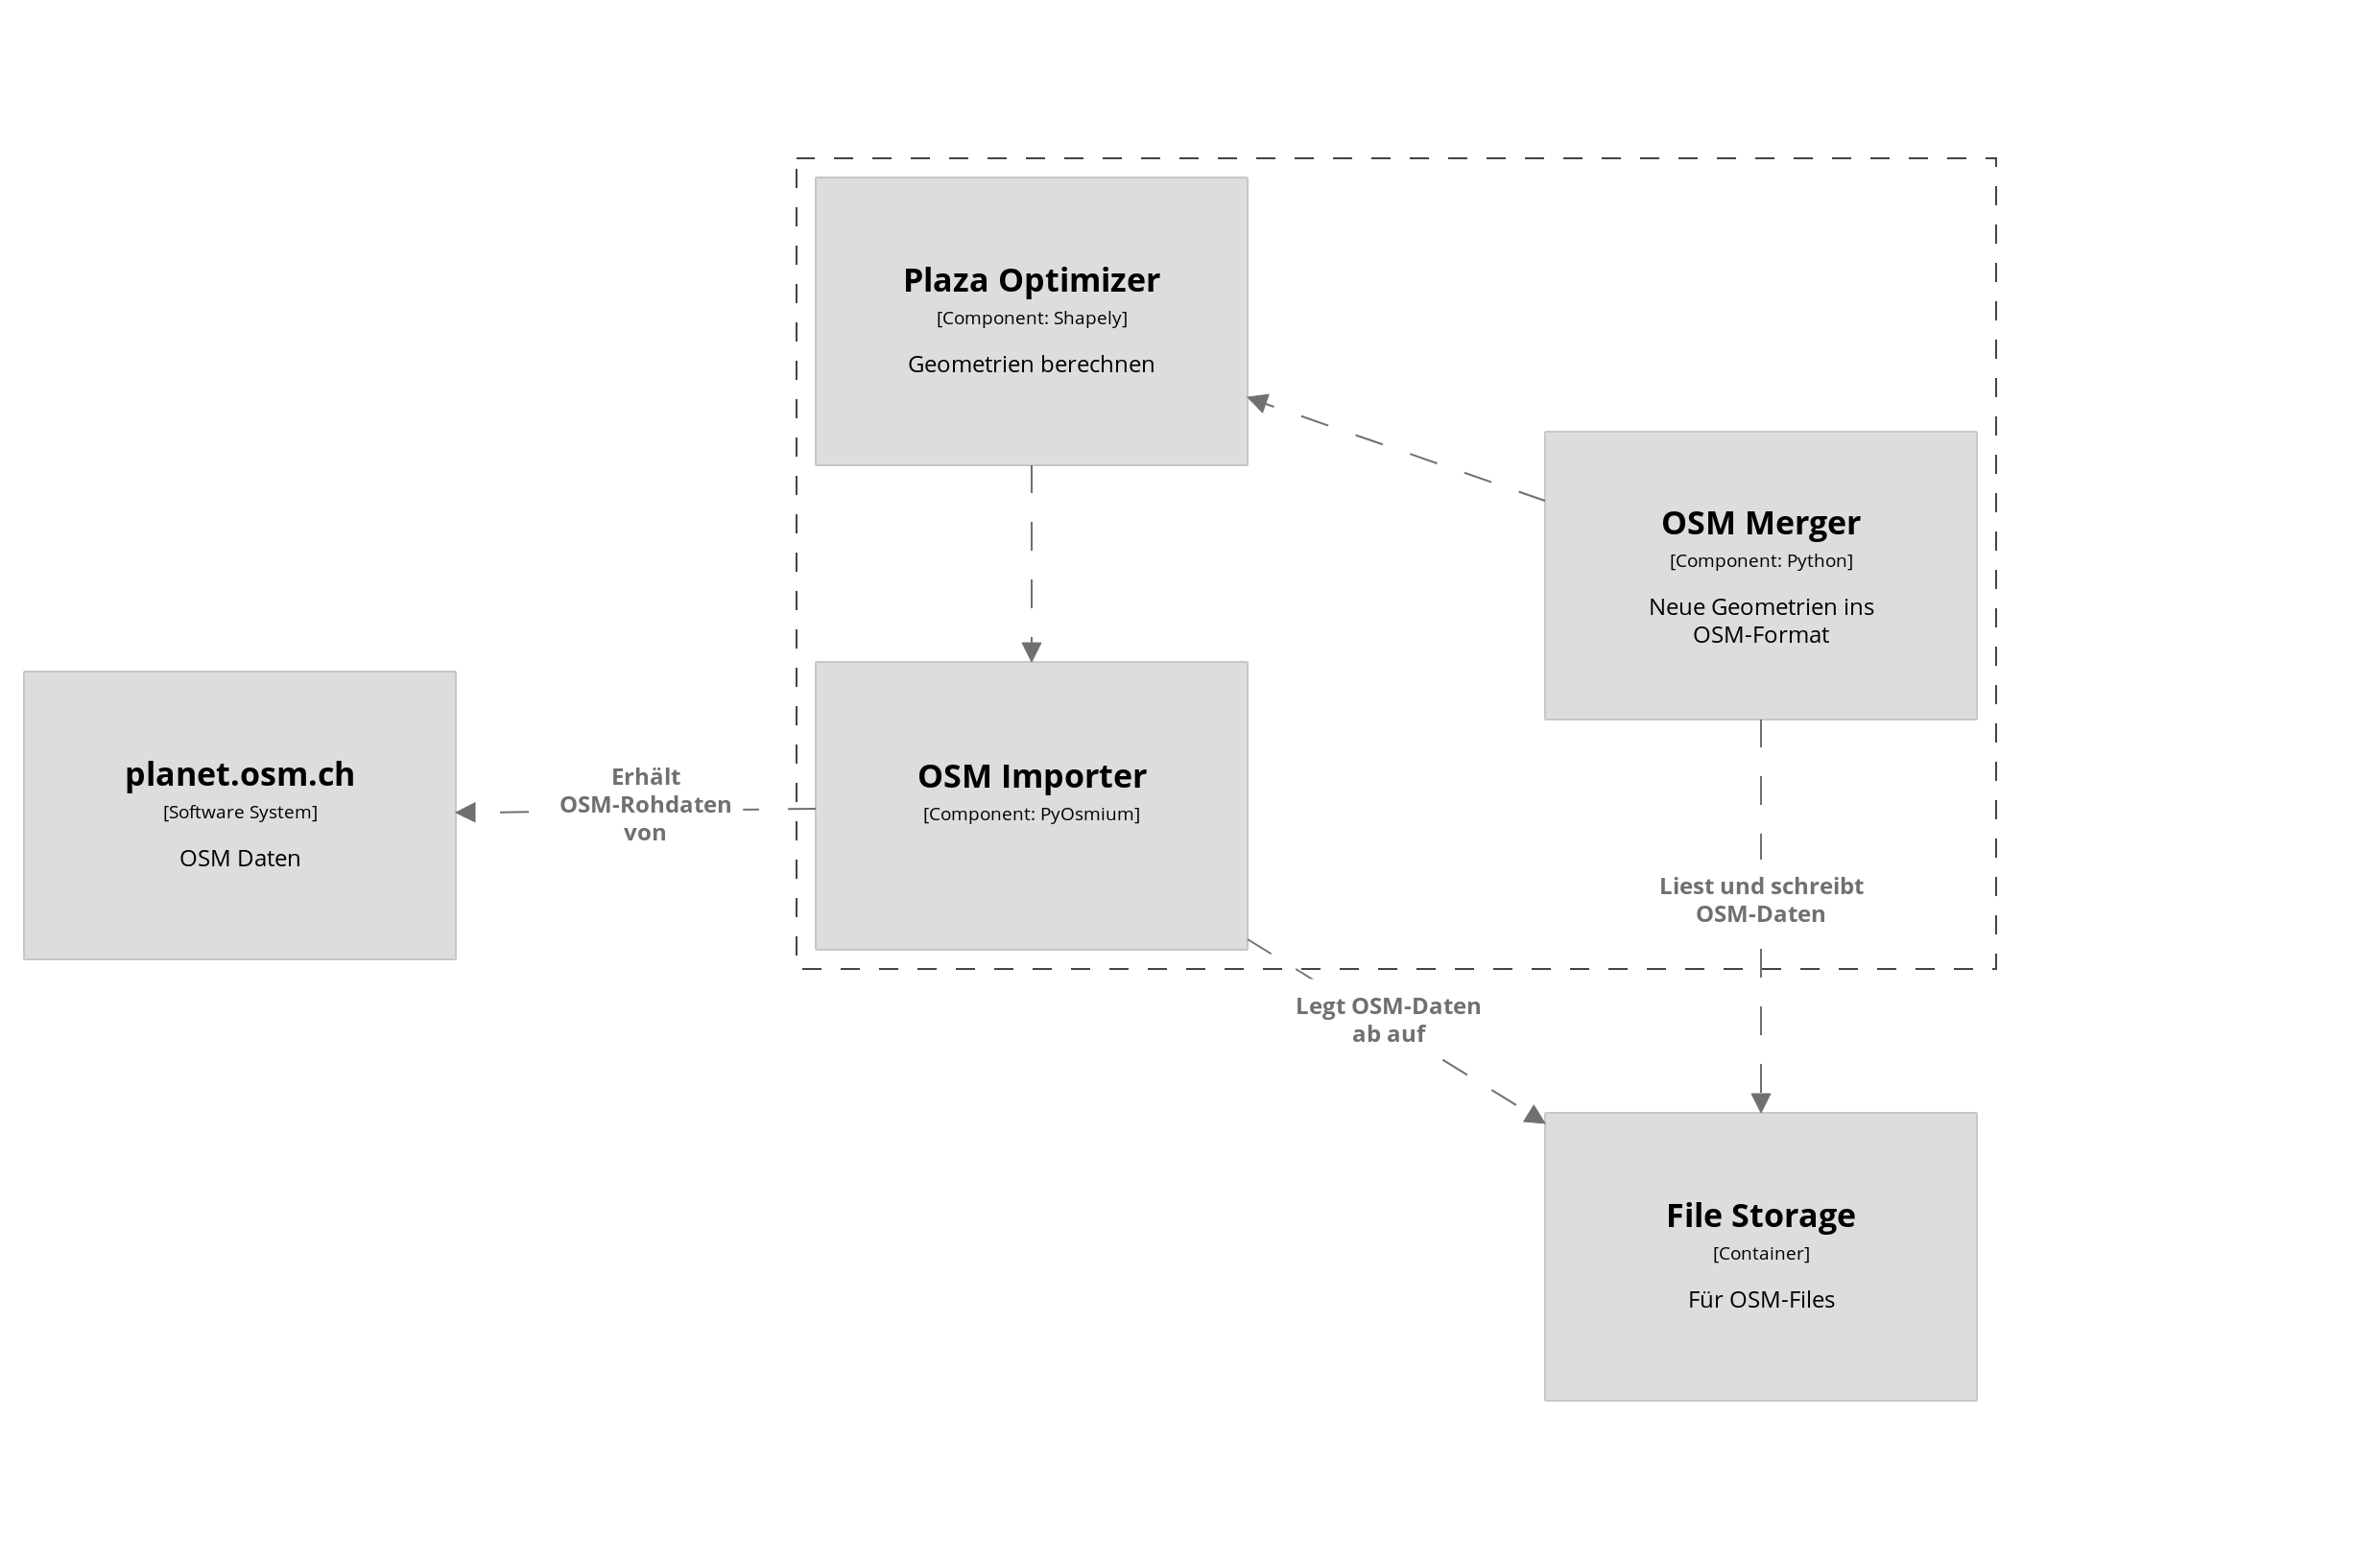
\includegraphics[width=1\linewidth]{projectdoc/img/component_diagram_plaza-vorverarbeitung.png}
\caption[Komponentendiagramm Vorverarbeitung]{Komponentendiagramm der Plaza Vorverarbeitung; Grafik erstellt mit \emph{Structurizr Express}\cite{structurizr}}
\label{fig:component_diagram_vorverarbeitung}
\end{figure}


\paragraph{OSM Importer}\label{par:OSM Importer}~\\
Für unser optimiertes Routing wird in regelmässigen Abständen der neueste \ac{OSM}-Datensatz \cite{osm_data_switzerland} der Schweiz geladen. Die \acs{OSM}-Importer Komponente liest das komplette für uns relevante Kartenmaterial (z.B. die Schweiz) als \ac{PBF} ein und sucht dabei nach Flächen, die wir bearbeiten wollen.

Dazu werden \emph{Osmium} und die dazugehörigen Python-Bindings \emph{pyOsmium}\cite{pyosmium} verwendet. Osmium erkennt automatisch Flächen aus \ac{OSM} Multipolygone oder Relationen. Mit einem eigenen Handler können wir dabei gleich das Einlesen des Files auf die für uns interessanten Flächen beschränken, wie in Listing \ref{osmium_import_code} gezeigt wird.

%TODO: In Implementation verschieben?

\begin{listing}[ht]
    \inputminted{python}{projectdoc/listing/osmium_handler.py}
    \caption[Einlesen OSM-Daten mit Osmium]{Einlesen von OSM Daten mithilfe von \emph{Osmium}; Filterung auf für uns relevante Flächen}
    \label{osmium_import_code}
\end{listing}

\paragraph{Plaza Optimizer}\label{par:Plaza Optimizer}~\\
Die mit Osmium importierten \ac{OSM}-Daten sind noch reine \ac{OSM}-Objekte, auf denen keine Geometrie-Berechnungen angewendet werden können. Dazu wird die Python-Library \emph{Shapely}\cite{shapely} verwendet. Shapely kann mit Geometrien umgehen und Algorithmen von \ac{GEOS} wie \code{intersection} und \code{contains} darauf anwenden.

Um die mit Osmium importierten Objekte in Shapely zu verwenden, werden diese ins \ac{WKB} Format übersetzt und Shapely übergeben, wie in Listing \ref{shapely_import_code} gezeigt.

\begin{listing}[ht]
    \inputminted{python}{projectdoc/listing/shapely_import.py}
    \caption[Einlesen OSM Objekte in Shapely]{Übergabe von Osmium-Objekten zu Shapely für die Weiterverarbeitung}
    \label{shapely_import_code}
\end{listing}



\paragraph{OSM Merger}\label{par:OSM Merger}~\\
Der OSM Merger ist dafür verantwortlich, unsere erzeugten Geometrien (Fusswege) wieder in das \ac{OSM}-Kartenmaterial einzupflegen, um es anschliessend der Routing-Engine zur Verarbeitung zum Routing-Graphen zu übergeben.

Die durch unseren Algorithmus erzeugten Wege durch Flächen (in Shapely Datenstrukturen) sollen nun wieder zurück ins \ac{OSM}-Format geschrieben werden. Die bisher erwähnten Libraries bieten eine solche Funktion leider nicht an. Auch sonst ist zum Zeitpunkt dieser Arbeit keine uns bekannte stabile Library dafür vorhanden. Die Erklärung dafür liegt wohl darin, dass beim Extrahieren der Geometrie (siehe Absatz \nameref{par:Plaza Optimizer}) alle Meta-Daten (z.B. Tags) von \ac{OSM} verloren gehen. Bei der umgekehrten Konvertierung (Geometrie zu \ac{OSM}) müssen also wieder Meta-Daten hinzugefügt werden. Diese Problematik kann ein generisches Konvertierungs-Tool nicht ohne weiteres lösen.

Für diese Komponente wird daher eine eigene Implementation geschrieben, die lediglich Wege aus Geometrien in ein \ac{OSM}-Format schreibt und mit den für uns relevanten Meta-Daten versieht.

In einem weiteren Schritt müssen unsere optimierten Wege in das bestehende Strassennetz eingebunden werden, damit die Routing-Engine diese beachtet. Dazu werden die Ein- und Ausgangspunkte der Wege im Polygon der Fläche referenziert. Dadurch werden sie auch topologisch mit den besthenden Strassen und Wegen verbunden, die das Polygon an diesen Punkten schneiden und einen Eintrittspunkt bilden.
% TODO: Begriff Eintrittspunkt definieren

\subsubsection{Plaza Routing}
\label{architektur:Plaza Routing}
Der Plaza Routing Container (siehe Abbildung \ref{fig:container_diagram}) ist für das Koordinieren und Verabeiten von Routing-Anfragen verantwortlich. Er bietet für das QGIS-Plugin eine API an. Mit Hilfe von search.ch (für ÖV-Routing) und der Routing-Engine (für Fussgänger-Routing) wird eine komplette Route mit Fahrplan erstellt und dem QGIS-Plugin übergeben.

\paragraph{nächste ÖV-Haltestellen finden}~\\
\label{architektur:nächste ÖV-Haltestellen finden}
Das grundlegende Ziel ist es von einem Startpunkt aus eine Destination zu Fuss und mit dem öffentlichen Verkehr zu erreichen. Dabei sollen die ÖV-Haltestellen in einem zu Fuss machbaren Umkreis berücksichtigt werden. Von diesen Haltestellen ausgehend wird das ÖV-Routing an die Zieldestination durchgeführt.

Für die Anforderung \ref{target:nächste ÖV-Haltestellen finden} bietet sich Overpass an. Overpass ermöglicht es über eine umfassende \ac{API} selektiv Daten von \ac{OSM} zu beziehen. Dabei besteht die Option, die Overpass \ac{QL} oder XML-Abfragen zu verwenden. Die Suche lässt sich nach allem einschränken, was der Mapper in den \ac{OSM}-Daten spezifizieren kann. So ist das Filtern nach Objekttyp, Keys, Tags, etc. unbeschränkt möglich und bietet so eine hohe Flexibilität. Overpass liefert die Resultate als JSON-Objekt oder XML. 

Für eine einfache Intergration in Python gibt es Overpass Wrapper. Dabei wurden zwei Libraries berücksichtigt, namentlich overpass-api-python-wrapper und OverPy. Die Libraries haben einen ähnlich häufigen Updatezyklus. Für beide wurde ein Proof of Concept implementiert, welcher die ÖV-Haltestellen im einem kleinen Umkreis vom Stadelhofen, Zürich, Schweiz abfragt.

Die Entscheidung fiel dabei auf OverPy. Ausschlaggebend war die ausführlichere Dokumentation und dass OverPy Klassen für Nodes, Relations, Way, Area, etc. und Hilfsfunktionen, welche das Ganze übersichtlich halten, anbietet. Bei overpass-api-python-wrapper besteht der Nachteil, dass das JSON-Resultat der Abfrage selber geparsed und verarbeitet werden muss.

\begin{listing}[ht]
    \inputminted{python}{projectdoc/listing/get_public_transport_stops_overpass.py}
    \caption{ÖV-Haltestellen von \acs{OSM} mit Overpass beziehen}
    \label{get_public_transport_stops_overpass}
\end{listing}

In Listing \ref{get_public_transport_stops_overpass} ist zu sehen, wie für eine Bounding Box, welche im Süden durch den minimalen Breitengrad, im Westen durch den minimalen Längengrad, im Norden durch den maximalen Breitengrad und im Osten durch den maximalen Längengrad begrenzt ist, die ÖV-Haltestellen abgefragt werden. Dabei wird die JSON-Response in Node-Objekte geparsed, welche weiterverwendet werden können. In diesem Beispiel wird für die Abfrage die erwähnte Overpass QL verwendet.

Es ist ebenfalls möglich, eine Umkreissuche mit \code{around} durchzuführen. Dies hat Performance-Nachteile und es gibt keine entscheidenden Gründe, warum es vorteilhafter sein sollte, wenn man einen Kreis statt ein Rechteck um einen Ausgangspunkt zieht.

\paragraph{Search.ch Anbindung}\label{architektur:Search.ch Anbindung}~\\

TODO

\subsubsection{Routing-Engine}
\label{architektur:Routing-Engine}

\paragraph{Evaluation Routing-Engine}~\\
\label{architektur:Evaluation Routing-Engine}
Eine Evaluation der heutig gängigen \ac{OSM}-Routing-Engines wurde in \cite{eval_routing_engine} ausgiebig durchgeführt. Bei unserer Evaluation beschränken wir uns auf \emph{Valhalla}\cite{valhalla} und \emph{Graphhopper}\cite{graphhopper}. Die Auswahl fiel auf diese zwei, weil \cite{eval_routing_engine} ergeben hat, dass Valhalla extrem schnell ist und Graphhopper Dijkstra und A* anbietet. So können wir zusätzlich analysieren, welcher Shortest-Path-Algorithmus sich für Flächen-Traversierungen besser eignet. Beide Routing-Engines bieten einen schnellen Einstieg und lassen sich in einigen Minuten problemlos aufsetzen.

Die beiden Engines werden an folgenden Kriterien gemessen:

\subparagraph{Infrastruktur-Integration}~\\
\label{architektur:Infrastruktur-Integration}
Es wird analysiert, wie einfach die Routing-Engine aufgesetzt werden kann. Ziel ist es, dass die Routing-Engine in einem eigenen Docker-Image (siehe \nameref{NFA:NFA01}) auf dem Server läuft.

\emph{Graphhopper} ist bereits als Docker-Image verfügbar und kann somit einfach auf einem beliebigen Server gestartet und verwendet werden.

\emph{Valhalla} ist als Ubuntu-\ac{PPA} verfügbar und lässt sich somit einfach auf einer Ubuntu-Distribution aufsetzen. Das Valhalla als Docker-Image verfügbar ist, muss noch umgesetzt werden.

\subparagraph{Applikation-Anbindung}~\\
\label{architektur:Applikation-Anbindung}
Damit die Komponente Plaza Routing mit der Routing-Engine kommunizieren kann, wird geprüft, wie einfach die Routing-Engines an eine Applikation angebunden werden können. 

\emph{Graphhopper} und \emph{Valhalla} bieten zusätzlich ein fertiges HTTP-Backend an, welches für das Routing genutzt werden kann. Somit können beide Routing-Engines auf die gleiche Art und Weise eingebunden werden.

% TODO kann man das bei Valhalla so sagen, oder ist es ein Frontend, welches missbraucht wird

\subparagraph{OSM-Daten-Integration}~\\
\label{architektur:OSM-Daten-Integration}
Die Komponente \nameref{architektur:Plaza Vorverarbeitung} generiert eigene \ac{OSM}-Daten. Damit das Fussgänger-Routing funktioniert, müssen die vorverarbeiteten \ac{OSM}-Daten der Routing-Engine übergeben werden. 

\emph{Graphhopper} und \emph{Valhalla} können beide beim Starten des HTTP-Backend eine \ac{OSM}-Datei übergeben werden.

% TODO: wollen wir noch prüfen, wie die Engines mit Änderungen umgehen können? Sprich muss alles neu importiert werden oder können sie mergen?

\subparagraph{Resultat}~\\
\label{architektur:Resulat}
Die beiden Engines unterscheiden sich in den oben definierten und analysierten Kriterien nur geringfügig. Die Entscheidung fiel zugunsten von Grahhopper. Ausschlaggebender Punkt war, dass Grahhopper bereits als Docker-Image verfügbar ist, was einen einfachen Aufbau der Infrastruktur ermöglicht.

\paragraph{Graphhopper}~\\
\label{architektur:Graphhopper}
% TODO wie kann Graphhopper genutzt werden?
TODO 



